\documentclass{article}
\usepackage[english]{babel}
\usepackage[utf8x]{inputenc}
\usepackage[T1]{fontenc}
\usepackage{graphicx}
\usepackage[colorinlistoftodos]{todonotes}
\usepackage[colorlinks=true, allcolors=tudelftblue]{hyperref} %sets hyperlink colour
\usepackage{caption}
\usepackage{subcaption}
\usepackage{xcolor}
\usepackage{roboto} % for Roboto Slab font
\usepackage{float}
\usepackage{titling} 
\usepackage{blindtext}\usepackage{titlesec}
\usepackage[square,sort,comma,numbers]{natbib}
\usepackage[colorinlistoftodos]{todonotes}
\usepackage{tikz}
\usepackage[siunitx]{circuitikz}
\usepackage{geometry}
\usepackage{sectsty}
\usepackage{amsmath}
\usepackage{tikzpagenodes}
\usepackage{booktabs}
\usepackage{listings}
\usepackage{minted}
\usepackage{svg}
\definecolor{darkgreen}{rgb}{0.0, 0.4, 0.0}
\definecolor{codegreen}{rgb}{0,0.5,0.1}
\definecolor{codegray}{rgb}{0.5,0.5,0.5}
\definecolor{codepurple}{rgb}{0.58,0,0.67}
\definecolor{backcolour}{rgb}{0.92,0.94,0.96}
\definecolor{keywordcolor}{rgb}{0.8, 0.2, 0.4}
\definecolor{titleblue}{rgb}{0.2, 0.4, 0.6}

\allsectionsfont{\color{titleblue}}
\lstdefinestyle{mystyle}{
    backgroundcolor=\color{backcolour},   
    commentstyle=\color{codegreen},
    keywordstyle=\color{keywordcolor},
    numberstyle=\tiny\color{codegray},
    stringstyle=\color{codepurple},
    basicstyle=\ttfamily\footnotesize,
    breakatwhitespace=false,         
    breaklines=true,                 
    captionpos=b,                    
    keepspaces=true,                 
    numbers=left,                    
    numbersep=5pt,                  
    showspaces=false,                
    showstringspaces=false,
    showtabs=false,                  
    tabsize=2
}
\lstset{style=mystyle}
\definecolor{tudelftdarkblue}{RGB}{12,35,64}
\definecolor{tudelftcyan}{RGB}{0,166,214}
\definecolor{tudelftblue}{RGB}{0, 118, 194}
\geometry{a4paper, margin=2cm}
\allsectionsfont{\color{black}} %sets colour for all headers
\usepackage{helvet}
\renewcommand{\familydefault}{\sfdefault}
\sectionfont{\fontfamily{RobotoSlab-TLF}\selectfont}
\setlength\parindent{0pt} %set no indent
%%%%%%%%%%%%%%%%%%%%%%%%%%%%%%%%%%%%%%%%%%%%%%%%%%%%%%%%%





\begin{document}

\begin{titlepage}
    \fontfamily{RobotoSlab-TLF}\selectfont 
%%%%%%%%%%%%%%%%%%%%%%%%%%%%%%%%%%%%%%%%%%%%%%%%%%%%%%%%%%UNCOMMENT THE FOLLOWING FOR LESS "PLAIN" TITLE PAGE (SELECT WITH MOUSE AND PRESS CTRL AND /)

    % \begin{tikzpicture}[remember picture,overlay]
    %     % Set seed for random number generator
    %     \pgfmathsetseed{4}
    %     % Define the text area to avoid
    %     \path (current page text area.south west) rectangle (current page text area.north east);
    %     % Adding circles spread over the entire page
    %     \foreach \x in {1,...,1000}
    %         \draw[tudelftdarkblue] (current page.south west) ++(rand*\paperwidth,rand*\paperheight) circle (rand*0.3);
    %     % Define coordinates for the corners of the white box
    %     \coordinate (A) at ([shift={(-8cm,12cm)}]current page.center);
    %     \coordinate (B) at ([shift={(8cm,-5cm)}]current page.center);
    %     % Draw the white background box
    %     \fill[white] (A) rectangle (B);
    %     % Adding equations as background features
    %     \node[anchor=center,rotate=20,text=tudelftcyan] at ([shift={(-7cm,-2cm)}]current page.center) {\fontsize{18}{22}\selectfont
    %     $\nabla^2 T - \frac{1}{\alpha}\frac{\partial T}{\partial t} = 0$};
    %     \node[anchor=center,rotate=-15,text=tudelftcyan] at ([shift={(5cm,-4cm)}]current page.center) {\fontsize{18}{22}\selectfont
    %     $\frac{\partial \rho}{\partial t} + \nabla \cdot (\rho \mathbf{v}) = 0$};
    %     \node[anchor=center,rotate=20,text=tudelftcyan] at ([shift={(6cm,4cm)}]current page.center) {\fontsize{18}{22}\selectfont
    %     $a^2 + b^2 = c^2$};
    %     \node[anchor=center,rotate=10,text=tudelftcyan] at ([shift={(7cm,-2cm)}]current page.center) {\fontsize{18}{22}\selectfont
    %     $E = \frac{\sigma}{\varepsilon}$};
    %     \node[anchor=center,rotate=-10,text=tudelftcyan] at ([shift={(-6cm,4cm)}]current page.center) {\fontsize{18}{22}\selectfont
    %     $F = ma$};
    %     \node[anchor=center,rotate=5,text=tudelftcyan] at ([shift={(-4cm,-5cm)}]current page.center) {\fontsize{18}{22}\selectfont
    %     $Q = -\frac{kA}{\mu} \frac{\Delta P}{L}$};
    % \end{tikzpicture}
%%%%%%%%%%%%%%%%%%%%%%%%%%%%%%%%%%%%%%%%%%%%%%%%%%%%%%%%%%
    \vspace*{3cm}
    
    \centering
    {\Huge \textbf{\textcolor{black}{Assignment Title}}}\\[1.5cm]
    \textsc{\LARGE Course Name}\\[0.5cm]
    \text{\large AESM3003}\\[2cm]
    
    {\Large \textbf{\textcolor{tudelftdarkblue}{Authors:}}}\\[0.5cm]
    \begin{tabular}{c}
        \Large \textcolor{tudelftdarkblue}{Author 1 (5381886)} \\
        \Large \textcolor{tudelftdarkblue}{Author 2 (1234567)} \\
        \Large \textcolor{tudelftdarkblue}{Author 3 (9876543)} \\
    \end{tabular}\\[2cm]
    
    {\Large \textcolor{tudelftdarkblue}{\today}}
    
    \vfill
    \begin{center}
        
\includegraphics[width=0.6\textwidth]{images/TU_delft_logo.jpg}
    \end{center}
\end{titlepage}

%%% Create a table of contents
\tableofcontents
\newpage

%%%Insert all the chapters
\addcontentsline{toc}{section}{Introduction}
\section*{Introduction}
Sample introduction text with a sample reference \cite{HussFarinotti2014}. Oh and here a sample figure with a sample caption, see \autoref{fig:random line}.

\begin{figure}[H]
\centering
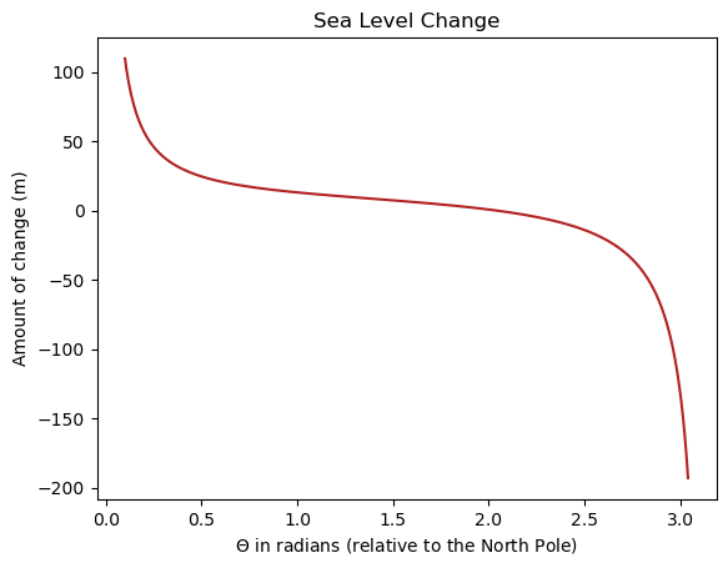
\includegraphics[width=0.6\textwidth]{images/Sample graph.png}
\caption{A graph of something.}
\label{fig:random line}
\end{figure}
\section{Methodology}
This section has a subsection.

\subsection{Some Math}
This subsection contains \autoref{eq:1}.
\begin{equation}
\label{eq:1}
    h(r) = \cfrac{Q}{2\pi T} \ln\left(\cfrac{r_i}{r_0}\right)+h_0
\end{equation}

\subsection{A circuit}
This subsection contains \autoref{circuit:useful_circuit}

\begin{figure}[H]
	\centering
	\begin{circuitikz}[american, scale=1]
		\draw
		(0,8) to [R, l=$3k\Omega$] (4,8)
		to [R, l=$4k\Omega$] (8,8)
		to [V, l=$12V$, invert] (8,4)
		to [R, l_=$6k\Omega$] (8,0)
		to [short] (0,0)
		to [V, l=$10V$, invert] (0,4)
		to [R, l=$2k\Omega$] (0, 8)
		(4,8) to [I, l=2mA, *-*, invert] (4,4)
		to [R, l=$6k\Omega$, *-*] (8,4)
		(4,4) to [R, l=$3k\Omega$] (4, 2) to [V, l=$8V$, -*] (4,0)
		(9, 4) to [open, v^>=$V_o$] (9, 0)
		;
	\end{circuitikz}
	\caption{A useful circuit}
	\label{circuit:useful_circuit}
\end{figure}


\input{Results}
\input{Discussion}


\newpage
\addcontentsline{toc}{section}{References}
\bibliographystyle{apalike}
\bibliography{ref}

\newpage
\appendix
\section{Additional graphs and data}

\section{Python code}
\begin{lstlisting}[language=Python]
import numpy as np
import pandas as pd
import matplotlib.pyplot as plt

#I forgot what this does
def heat_produced(filename, time_data, plot_cols):
    heat = time_data['PRD1 : energy (kJ/day)']*-1
    time = time_data['Time (yrs)']
\end{lstlisting}

\end{document}






%All other official TU Delft colours
\definecolor{donkerblauw}{RGB}{12, 35, 64}
\definecolor{turkoois}{RGB}{0, 184, 200}
\definecolor{blauw}{RGB}{0, 118, 194}
\definecolor{paars}{RGB}{111, 29, 119}
\definecolor{roze}{RGB}{239, 96, 163}
\definecolor{framboos}{RGB}{165, 0, 52}
\definecolor{rood}{RGB}{224, 60, 49}
\definecolor{oranje}{RGB}{237, 104, 66}
\definecolor{geel}{RGB}{255, 184, 28}
\definecolor{lichtgroen}{RGB}{108, 194, 74}
\definecolor{donkergroen}{RGB}{0, 155, 119}
%You can use these to change the hyperlink colour or the colour of the header or whatever. Glück Auf!
